\section{並列削除アルゴリズム}\label{section:delete}

並列削除のための基本的な着想は,扁平化操作を,削除すべき節点を下降さ
せるために利用することである.これまでは,扁平化操作はもっぱら,再度アク
セスしそう
な節点を浮上させるために用いられてきた.ここで重要なことは,削除対象の
節点以外は高々${\rm O}(1)$レベルしか下降させないようにすることである.
以下では,$z$を削除対象の節点とする.

まず,根節点が削除対象節点$z$である場合を考える.この場合,zippingと呼ぶ
操作によって
それを``容易に''削除できる場所まで下降させる.節点が``容易に''削除でき
るとは,その左部分木,右部分木,左部分木の右部分木,右部分木の左部分木の
いずれかが空であることである.根節点の下降によって,その左部分木と
右部分木の縫い合せが起きる.
%
% これが言葉の由来である.

\begin{enumerate}
% \medskip\noindent (a)
\item[(a)]
``容易に''削除できる場合:図\ref{figure:delete}(a1)または(a2)
のように変形する.


% \begin{adjustvboxheight}
\begin{figure*}[t]
  \centerline {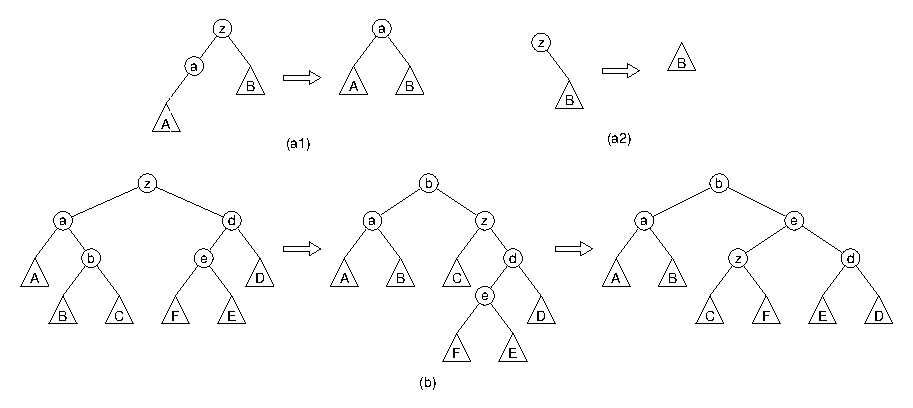
\includegraphics {images/fig4.eps}}
\caption{後続操作をブロックしない削除アルゴリズムの1ステップ}
\label{figure:delete}
\end{figure*}
% \end{adjustvboxheight}

% \medskip\noindent (b)
\item[(b)]
``容易に''削除できない場合:図\ref{figure:delete}(b)のように
zig-zagを施し,そ
の結果できる$b$の右部分木に,(一つめとは左右対称な) zig-zagを施す.

\noindent
4回の回転で$z$は2レベル下降する.$z$の新たな部分木$C$と$F$
は,同じレベルにとどまる.それ以外の節点も高々1レベルしか下降
しない.$z$を根とする新たな部分木に対して再帰的に削除操作を行なうが,$z$の子孫
でない節点がそれによってさらに下降することはない.
\end{enumerate}

% \medskip
図\ref{figure:zipping}に,根節点$z$の削除による木の形状の変化を示す.
\begin{figure*}[t]
  \centerline {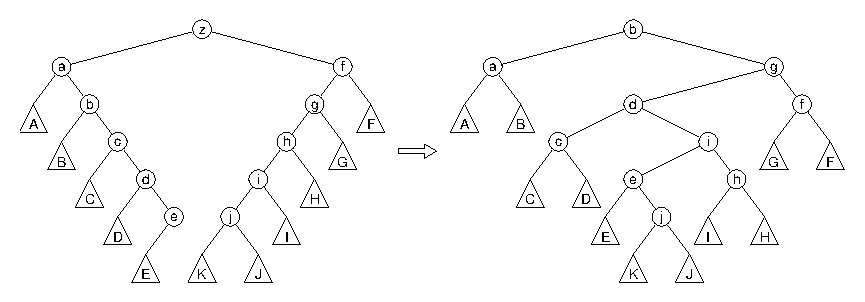
\includegraphics {images/fig5.eps}}
\caption{Zippingによる節点$z$の削除}
\label{figure:zipping}
\end{figure*}

削除対象節点$z$が根であるとは限らない場合は,まず第\ref{section:update}節の
方法で$z$を探索する.これは根から$z$に至るパスを短縮する効果をもつ.つぎ
に,$z$をzippingによって下降させて削除する.

Zipping操作はパスの短縮を行なわないが,アクセスした節点は浮上させ
るという原則にしたがうならば,zippingに先だって,左部分木の最大要素に至
るパスと右部分木の最小要素に至るパスをそれぞれトップダウンの半扁平化
(zig-zig (図\ref{figure:update}(c)) の繰返し)によっ
て短縮すればよい.この短縮化はzippingと並行して行なうことができる.

Zippingは更新操作と異なり,各節点のキー値を読むことなく木を下降する.
またzippingは,木$T_1$と木$T_2$ ($T_1$のど
のキーも,$T_2$のどのキーよりも小さいものとする)とのトップダウン併合操作
にも応用できる.すなわち,新たな節点(キーは任意)を調達し,その左部分木
を$T_1$,右部分木を$T_2$として一つの木を構成した
のち,調達した根節点を消去すればよい.
